\documentclass{beamer}
\beamertemplatenavigationsymbolsempty
\usecolortheme{beaver}
\setbeamertemplate{blocks}[rounded=true, shadow=true]
\setbeamertemplate{footline}[page number]
%
\usepackage[utf8]{inputenc}
\usepackage[english]{babel}
\usepackage{amssymb,amsfonts,amsmath,mathtext}
\usepackage{subfig}
\usepackage[all]{xy} % xy package for diagrams
\usepackage{array}
\usepackage{multicol}% many columns in slide
\usepackage{hyperref}% urls
\usepackage{hhline}%tables
% Your figures are here:
\graphicspath{ {fig/} {../figs/} }

%----------------------------------------------------------------------------------------------------------
\title[\hbox to 56mm{Feature generation}]{Differentially private modification of sign-SGD}
\author[A.\,Yu.~Kravatskiy]{Alexey Kravatskiy}
\institute{Moscow Institute of Physics and Technology}
\date{\footnotesize
\par\smallskip\emph{Course:} My first scientific paper\par (Strijov's practice)/Group 205 %821, 813
\par\smallskip\emph{Expert:} A.\,N.~Beznosikov
\par\smallskip\emph{Consultant:} S.\,A.~Chezhegov
\par\bigskip\small 2025}

%----------------------------------------------------------------------------------------------------------
\begin{document}
%----------------------------------------------------------------------------------------------------------
\begin{frame}
\thispagestyle{empty}
\maketitle
\end{frame}
%-----------------------------------------------------------------------------------------------------
\begin{frame}{Goal of research}
% goal: private algorithm for federated learning
% problem: dp-sign sgd with sigma
% solution: a privacy accountant that makes dp-sign converge
\end{frame}
%-----------------------------------------------------------------------------------------------------
\begin{frame}{One-slide talk}
% light convergence slide
Please comment all slides but this one if you make the One-slide talk.

\begin{columns}[c]
\column{0.6\textwidth}
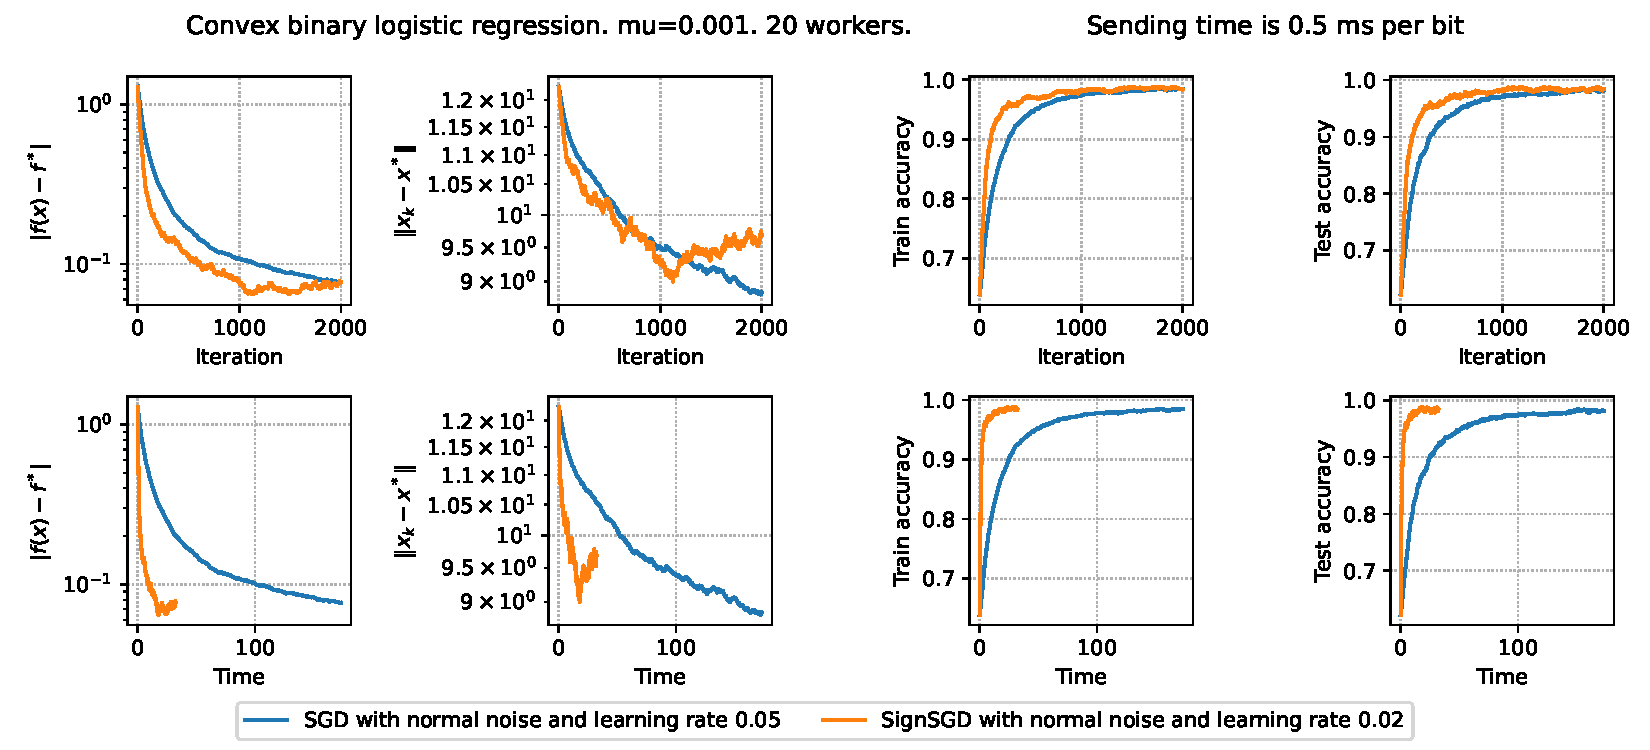
\includegraphics[width=1.0\textwidth]{sgd_vs_sign_sgd}
    Column 1
\column{0.4\textwidth}
    Column 2
\end{columns}

\bigskip
The {\color{red}message}.
\end{frame}

%-----------------------------------------------------------------------------------------------------
\begin{frame}{Literature}
% Jin 2020
% Mironov 2017
% Mironov 2019
\end{frame}
%----------------------------------------------------------------------------------------------------------
\begin{frame}{Differential Privacy}
% defintion of differential privacy
\end{frame}
%-----------------------------------------------------------------------------------------------------
\begin{frame}{Renyi differential privacy}
% Renyi differential privacy
% conversion to common privacy
% composite theorem
\end{frame}
%-----------------------------------------------------------------------------------------------------
\begin{frame}{Criterion of a private algorithm}
% bound on epsilon R
\end{frame}
%-----------------------------------------------------------------------------------------------------
\begin{frame}{Sample Gaussian Mechanism}
% definition
% expression on Er with numerical techniques
\end{frame}
%----------------------------------------------------------------------------------------------------------
\begin{frame}{Solution}
\begin{columns}[c]
\column{0.6\textwidth}
    Column 1
\column{0.4\textwidth}
    Column 2
\end{columns}
\end{frame}
%----------------------------------------------------------------------------------------------------------
\begin{frame}{Computational experiment}
% big chart
\end{frame}
%----------------------------------------------------------------------------------------------------------
\begin{frame}{Conclusion}
    \begin{block}{dp-sign SGD}
    \begin{itemize}
        \item with Poisson sampling $q = 1/n$ 
        \item is $(10, 1/n^{1.1})$ differentially-private
        \item empirically converges on logistic regression problem even with heavy-tailed noise
    \end{itemize}
    \end{block}
    Now we have to provide theoretical guarantees of convergence.
\end{frame}
%----------------------------------------------------------------------------------------------------------
\end{document} 